% Search for all the places that say "PUT SOMETHING HERE".

\documentclass[11pt]{article}
\usepackage{cube,amsmath,textcomp,amssymb,geometry,graphicx,enumerate,longtable}
\usepackage{longtable}
\usepackage{array}
\newcolumntype{L}[1]{>{\raggedright\let\newline\\\arraybackslash\hspace{0pt}}m{#1}}

\usepackage{multirow}

\def\Session{Fall 2021}

% \title{Syllabus}
\author{\Name, SID \SID}
% \pagestyle{headings}
\date{}

\newenvironment{qparts}{\begin{enumerate}[{(}a{)}]}{\end{enumerate}}
\def\endproofmark{$\Box$}
% \newenvironment{proof}{\par{\bf Proof}:}{\endproofmark\smallskip}

\textheight=9in
\textwidth=6.5in
\topmargin=-.75in
\oddsidemargin=0.25in
\evensidemargin=0.25in

\begin{document}
\maketitle
\title{Course Syllabus}
\centerline{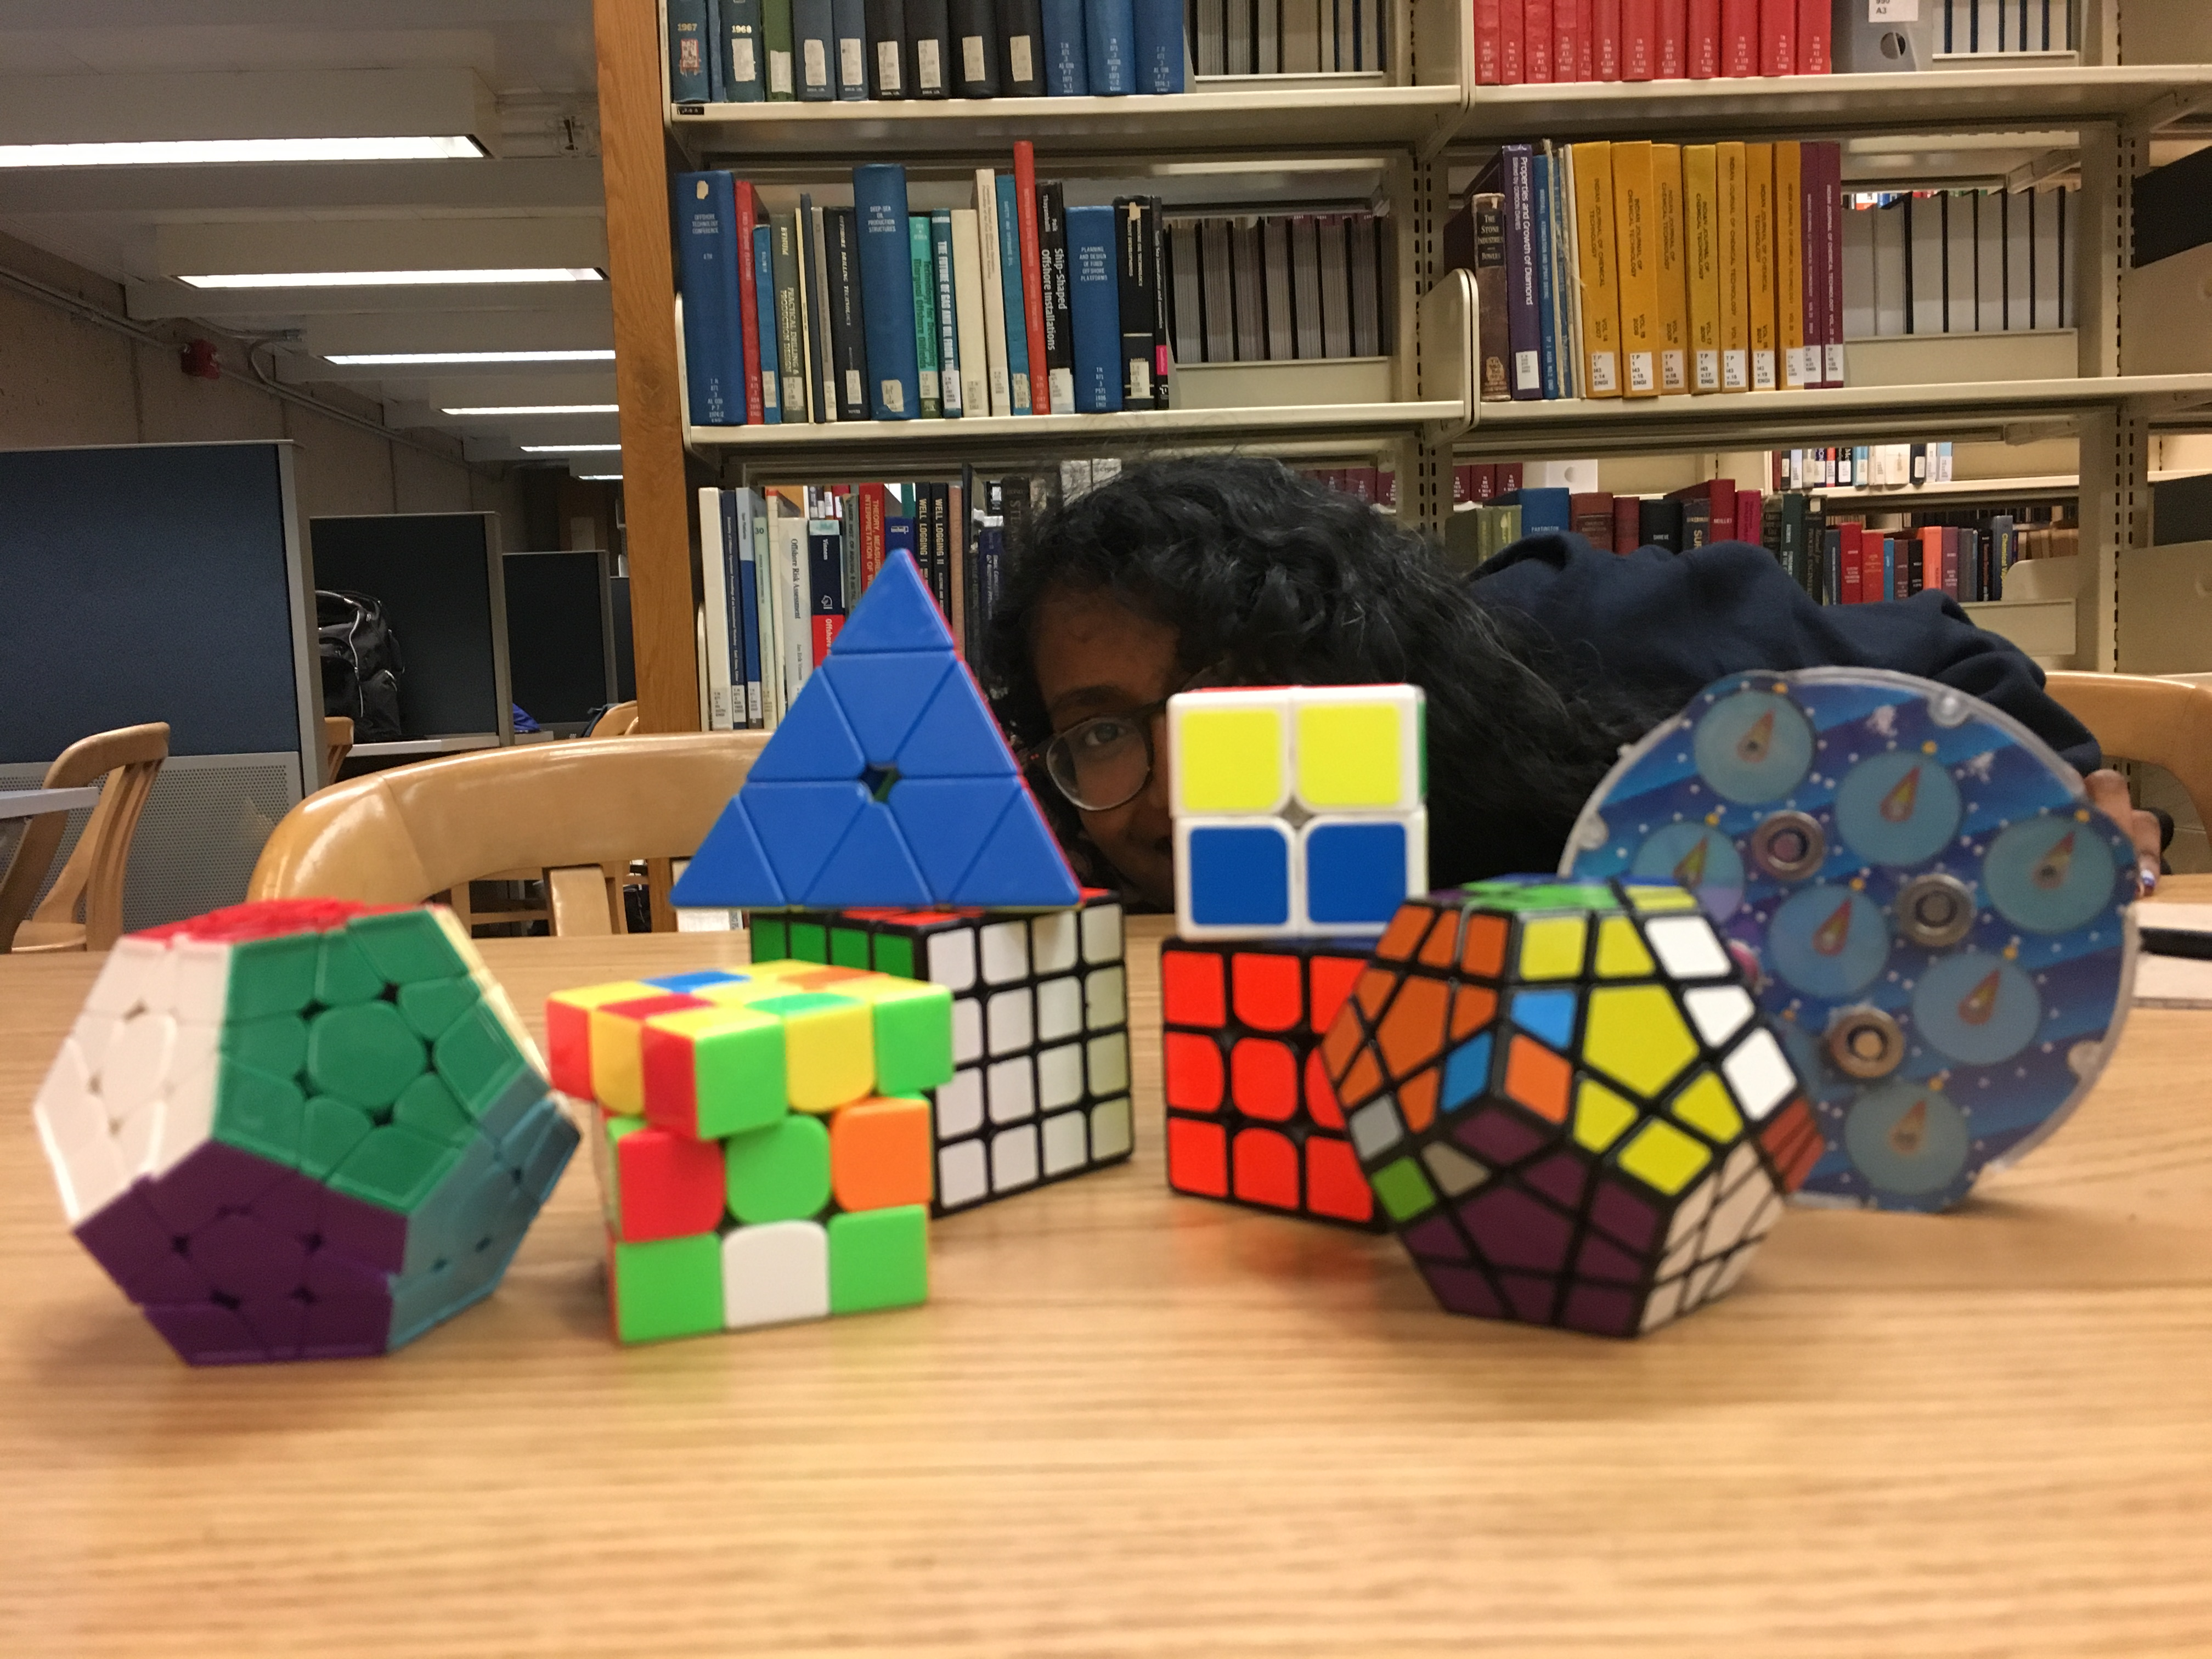
\includegraphics[width=10cm]{5.JPG}}

$\textbf{Semester}$: Fall 2021\\
$\textbf{Room}$: 390 Hearst Mining Memorial\\
$\textbf{Time}$: Monday 5-7 PM (Beginners 5-6 PM, Advanced 6-7 PM)\\
$\textbf{Starting Date}$: September 14th\\
$\textbf{Ending Date}$: December 2nd\\
$\textbf{Facilitators}$: Aaron Sun (aaronsun2000@berkeley.edu), An Le (anl2002@berkeley.edu) \\
$\textbf{Faculty Sponsor}$: Peng Zhou\\
$\textbf{Office Hours}$: After class/By appointment/Instructor Email \\
$\textbf{Grading}$: 1 unit P/NP only

\section*{Objective}
In this DeCal you will learn how to solve the Rubik’s Cube (Beginner section) or how to solve it much more quickly and efficiently (Advanced section), using concepts from group theory as they apply to the cube. Learning to solve the Rubik's cube is a good way to build intuition for topics in abstract algebra without needing to worry too much about all the technical details, whether you plan to study mathematics or not. You will leave with better problem solving abilities, improved understanding on the history and mathematics of the Rubik’s Cube, improved hand-eye coordination, increased finger dexterity, and a cool party trick!


\section*{Format}
The format of this class will be a combination of lecture and group instruction, with a heavy emphasis on the latter. At the beginning of each class, we will give a brief overview of the lesson and then break into groups for the remainder of the hour. In these groups, you will practice the lessons taught during lecture with personal guidance from your group instructor (you will stay with the same instructor for the entire semester).

\section*{Content}
In the Beginner section, we will be teaching the Layer-By-Layer method, which involves solving the cube “from the ground up”. In the last few weeks of class, we will be holding instruction on various topics such as solving the cube faster and solving other puzzles, or even solving the cube blindfolded! If you finish the basic curriculum early on, you will have the opportunity to learn more of these topics from your instructor.

In the Advanced section, we will be teaching the CFOP method, a more advanced version of the Layer-By-Layer method that many people learn. In addition, since more one-on-one instruction is available in the Advanced section, the class is much more flexible. If you have a particular cube-related topic that you would really like to learn, chances are there is an instructor who can teach it to you while or after you learn the regular curriculum. Just be aware that we expect you to fully learn the CFOP method that we teach, and utilize it in your solving (during the final and competition). Anything after that is up to you.

In both sections, students will learn how solving the Rubik's cube is an application of group theory and the underlying mathematics taking place with each move. More specifically, we will discuss how the Rubik's cube is an example of a group and explore what implications this has on the movement of pieces and potential permutations the cube can take. Algorithms we teach will be built up from the basics using easy to understand mathematical concepts, which makes them easier to remember as well as giving a deeper understanding of how the cube works. Of particular importance are the concepts of conjugation and commutators. Students will also gain familiarity with standard cube notation, which is taken from the notation of group theory. Particular emphasis is placed on notation in the advanced section.

\section*{Workload}
\subsection*{Come to class}
This is mandatory, as we will introduce a new topic each week and move fairly quickly through the steps. If you miss a class, you will be behind on material. Attendance will be taken weekly by your instructors — if you must miss a class, please let your instructor know ahead of time (unless it’s an emergency). We will allow 3 absences, either excused or unexcused. If you have 4 absences, we will fail you.

\subsection*{Work outside of class}
Besides coming to class, you will need to practice on your Rubik’s Cube outside of class. This can be as little as 15 minutes per day, but obviously the more the better. Practice hones your skills and helps you identify problem areas that you can then ask your instructor about during class. If you practice consistently, you will easily be able to learn the regular curriculum within the first few weeks.  Additionally, you must read articles assigned every other week to further supplement your learning experience.

\subsection*{Do the readings}
In both sections, there will be required biweekly readings consisting of articles and short documents on various aspects of the Rubik’s Cube.  These articles will mainly highlight the mathematics and the history of the Rubik’s Cube and similar puzzles. Students will be required to do short exercises related to the readings.

\subsection*{Pass the tests}
\hspace{\parindent} \textit{\textbf{Part 1}} \\
\underline{Solve the Cube}: For the Beginner section, this means solving the cube once in under 5 minutes or under 250 moves. You will have up to 5 attempts, if necessary. If you successfully solve the cube on your first try, you pass the test and do not have to complete your remaining attempts (unless you want to).

For the Advanced section, this means solving the cube in under 1 minute 15 seconds or under 85 moves at least once. You also must complete all five solves to pass.

\textit{\textbf{Part 2}} \\
\underline{Take-home Exam}: Additionally, for both sections, there will be a take-home final consisting of short answer and multiple-choice questions.
The take-home exam will test students on the semester’s readings and mathematical content, with emphasis on basic computations and permutation groups.


\subsection*{Participate in a competition}
\textit{(Required only for advanced, although beginners are welcome as well!)} - Advanced students are expected to register and compete in a competition during the semester. Competitions can be found at the following links:
\[www.cuberslive.com/tpc/\]
\[www.cubingathome.com/\]
The Bay Area traditionally holds 3-5 competitions per semester in Berkeley, South Bay, etc. through the World Cube Association, but unfortunately in-person competitions are cancelled for the time being. If it turns out that you are not available for any of the online competitions, please let us know as early as possible and we will work something out.\\
\textbf{Note:} You must complete all of these requirements to pass this class. Failure to do so will result in a grade of NP (no pass).


\section*{Grading}
In addition to completing all the mandatory requirements for both the Beginner’s and Advanced section, a total cumulative grade of 70\% must be achieved in order to pass the class. Note that students will receive an NP if they miss 3 or more classes. The breakdown is as follows:
\begin{center}
\begin{tabular}{|l|l|}
\hline
Solve Cube             & 40\% \\ \hline
Papers \& Assignments* & 30\% \\ \hline
Take-home Exam         & 30\% \\ \hline
\end{tabular}
\end{center}
\begin{footnotesize}
*Short readings + problem sets will be assigned throughout the semester. Readings are TBD. 
\end{footnotesize}

\section*{Prerequisites and Materials}
For the Beginner section, the only prerequisite is that you have your own Rubik’s Cube to practice on. You will not be allowed to share with any other students. No other experience with the Rubik’s Cube or other puzzles is necessary, as we will teach you how to solve it from scratch.

For the Advanced section, you will also need your own Rubik’s Cube to practice with. You will not be allowed to share with any other students. In addition, you must already know how to solve the cube using any method before the first day of class. We would prefer that you know the layer-by-layer method; if you know another method, let us know so that we can tailor the course to meet your needs. This ensures that you have some experience with the cube and that you have some basic intuition with respect to how the cube works.

We will have cubes available for purchase for \$10 at the beginning of the course. Cubes can be purchased from several online retailers, the largest of which is \textit{thecubicle.com} (based in New York).

If you are confused on which section you belong in, talk to one of the facilitators during the first class, and we will determine which section you should take.

\section*{Other Policies}
In order for the class to proceed smoothly, it should be free of any distractions: \\
Cell Phones - should be left on silent.\\
Tardiness - you should show up by 10 minutes after the hour (Berkeley time).\\
DSP Accomodations - come talk to us or send the instructors an email.\\
If you would like to request special accommodations, particularly if you will need extra time to solve the cube, please contact the instructors during the first two weeks of the course and we will be happy to assist you.

\section*{Enrollment}
Deadline to fill out the application listed on the DeCal website — September 8th.\\
Note the application includes choosing either the beginner or the advanced section.\\
We will select $\sim$130 applicants and send them an email with the CCNs on September 10th.\\
CCNs will be made available to everyone on the DeCal website after the first class, which will be on September 14th.\\
The CCNs will be taken off of the DeCal website on October 1st.\\
Beginner’s tests will be held on the last two weeks of class, November 19th and December 2nd.\\
Advanced tests will be held on the last week of class. More information will be presented in class.

See the DeCal website for further details.

\section*{Schedule}
Note: Teaching topics are roughly listed and depend on your instructor.
\begin{center}
\begin{longtable}{|L{1cm}|L{4.6cm}|L{4.6cm}|L{4.6cm}|}
\hline
Week \# & Beginner &  Advanced 	& Readings/Additional HW* \\ \hline
1  & Meet your instructor, intro to the cube and Step 1: Cross & Meet your instructor, diagnostics + planning, intro to CFOP & Obtain a cube \\ \hline
2  & Step 2: First layer & Intro to first two layer solving & Cube combinatorics \\ \hline
3  & Step 3: Middle Layer Checkpoint quiz: First layer & Two look OLL & Learn about the WCA Advanced: Register for a competition (beginners welcome) \\ \hline
4  & Steps 4-5: Orientation of the last layer & Two look PLL & Permutation cycle notation \\ \hline
5  & Steps 6-7: Finishing the cube & Various shortcuts throughout the solve & Checkpoint quiz 1: Solve entire cube (with F2L techniques for advanced) \\ \hline
6  & Buffer/review week. Perfect solving the cube from start to finish & Advanced cross solving and fingertricks & Groups and conjugation \\ \hline
7 & Intro to some simple shortcuts & Inspection, cutting rotations and efficiency & Checkpoint quiz 2: Solve the cube (Reconstructing the solve for advanced) \\ \hline %Lecture day: Topic TBA & Lecture day: Topic TBA & Non-Abelian groups and commutators \\ \hline
8 & Lecture day: Topic TBA & Lecture day: Topic TBA & Non-Abelian groups and commutators \\\hline %Intro to some simple shortcuts & Inspection, cutting rotations and efficiency & Checkpoint quiz 2: Solve the cube (Reconstructing the solve for advanced) \\ \hline
9 & Advanced cross solving & Easy algorithms to learn  & Subgroups and Lagrange's theorem\\ \hline
10 & Intro to four look last layer algorithms & Orientation for future learning: how to improve after the class is over & Finish the readings \\ \hline
11 & Review week & Review week 1 & Complete Take-home Exam \\ \hline
12 & Cube solving part 1 & Review week 2 & \\ \hline
13 & Cube solving part 2 & Cube solving & \\ \hline
\end{longtable}
\end{center}

\begin{footnotesize}
*Homework is the same for both sections unless listed otherwise. Failure to pass both checkpoint quizzes may result in a NP in the course.

In addition to the listed assignments, students are expected to practice all topics taught so far on their own for 2-3 hours a week. Students will be tested every week on the previous week’s material to make sure they are practicing outside of class. 
\end{footnotesize}

\subsection*{Checkpoint Quiz 1}
This in-class quiz will be used to measure the progress of students and ensure that they are practicing outside of class time. Students are expected to be able to solve the cube start to finish without aid from their instructors. However, using a sheet of algorithms is permitted. For advanced students, they must be able to solve the entire cube using the F2L technique taught and not the Beginner’s method


\subsection*{Checkpoint Quiz 2}
The second in-class quiz will be used to check whether students have fully memorized the algorithms required for solving the cube. Beginner students are expected to be able to completely solve the cube in under 10 minutes and have all the algorithms memorized. Advanced students are required to be able to write down a reconstruction of their solves using standard notation and are required to have memorized the baseline OLL and PLL algorithms. Advanced students are encouraged to learn the remaining algorithms, but it is not required.


\subsection*{Take-home Exam}

The exam will cover the readings assigned up to Week 10. The topics covered in the readings include but are not limited to: the mathematics behind the Rubik’s cube (particularly group theory), the history of the Rubik’s cube, and algorithm intuition and development. The exam will be due one week after the readings are assigned, and will have an emphasis on the mathematical readings. The readings will be posted shortly after the beginning of the course to give students plenty of time to read them ahead of time.


\end{document}